\section{Evaluation}

We address the following questions in our evaluation:
\begin{enumerate}
\item How does NOPaxos's performance on a cloud platform compare to its performance on dedicated hardware?
\item How do the modifications to NOPaxos required for a cloud platform affect its ability to scale?
\end{enumerate}

\begin{figure}[tp]
\centering
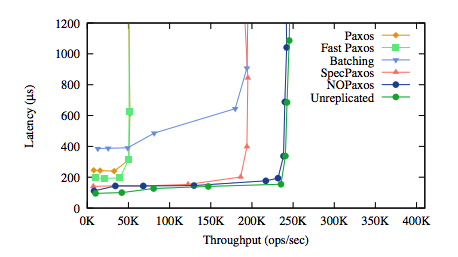
\includegraphics[scale=0.5]{figures/figure_5.png}
\caption{Original Figure 5 in \cite{nopaxos}, showing latency vs. throughput comparison for NOPaxos and other protocols}
\end{figure}

\begin{figure}[tp]
\centering
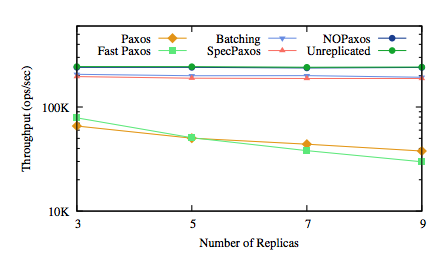
\includegraphics[scale=0.5]{figures/figure_8.png}
\caption{Original Figure 8 in \cite{nopaxos}, showing maximum throughput with increasing number of replicas}
\end{figure}

\subsection{NOPaxos: Dedicated Hardware}

\cite{nopaxos} shows that on dedicated hardware using a hardware middlebox sequencer, NOPaxos on achieves a throughput within 2\% and latency within 16 microseconds of an unreplicated system, better than any existing consensus protocol. NOPaxos continues to maintain a throughput comparable to an unreplicated system as the number of replicas increases. The throughput and latency results are presented in Figure 5 of \cite{nopaxos} and the scaling results in Figure 8, both included here for reference (Figures 1 and 2). Note that because we use the end-host sequencer implementation, our NOPaxos results are more directly comparable to Figure 6 of \cite{nopaxos}; however, Figure 6 shows that the performance of NOPaxos with an end-host sequencer is very similar to that of NOPaxos with a hardware middlebox sequencer, with comparable throughput and only a slight increase in latency; therefore we include Figure 5, as it shows the performance of NOPaxos in relation to the other evaluated consensus protocols. 

\subsection{NOPaxos: Cloud Platform}

\begin{figure}[tp]
\centering
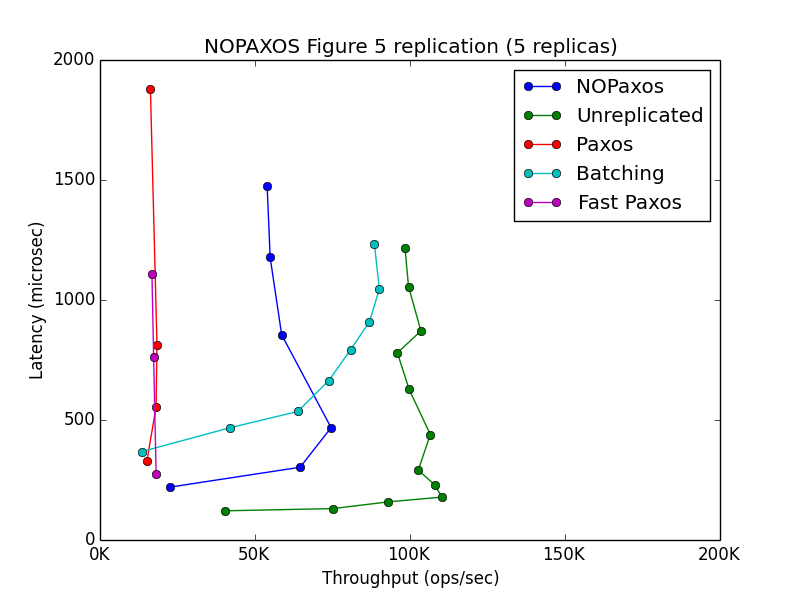
\includegraphics[scale=0.5]{figures/Figure5-5.png}
\caption{Reproduction of Figure 5 in \cite{nopaxos} with 5 replicas, showing latency vs. throughput comparison for NOPaxos and other protocols}
\end{figure}

\begin{figure}[tp]
\centering
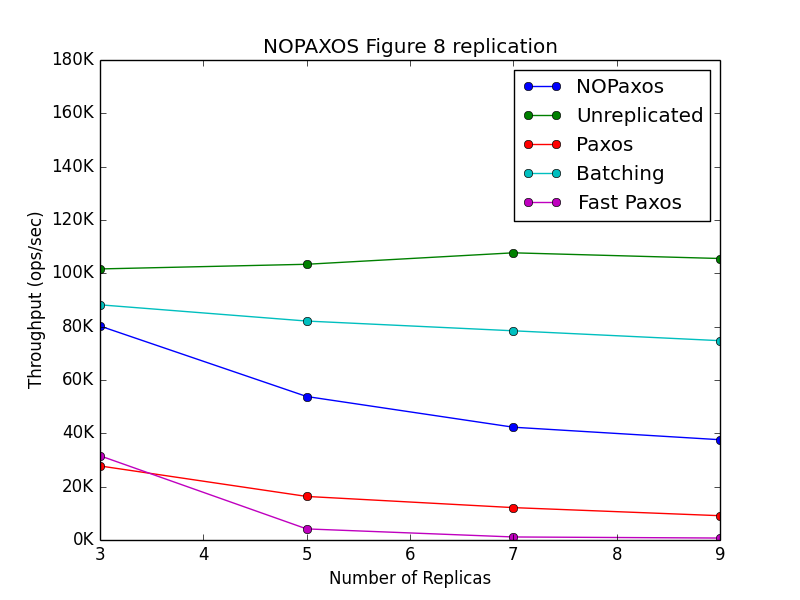
\includegraphics[scale=0.5]{figures/Figure8.png}
\caption{Reproduction of Figure 8 in \cite{nopaxos}, showing maximum throughput with increasing number of replicas}
\end{figure}

\textbf{Throughput/Latency: }We present the throughput and latency results of our experiments in Figure 3, preserving the formatting of the original paper's Figure 5 for comparison. We can see that the relative performances of Paxos, Fast Paxos, Batching (Paxos with Batching), and Unreplicated on the cloud platform reflect the results of the dedicated hardware experiments performed by the authors. Paxos and Fast Paxos both have very low maximum throughput, although Fast Paxos has slightly lower latency, and Batching gets closer to the throughput of Unreplicated, although with much higher latency.

NOPaxos, however, has a noticeable difference in its performance relative to the other consensus protocols when run on a cloud platform rather than dedicated hardware. Although it continues to achieve considerably lower latency than the other (replicated) protocols prior to reaching its maximum throughput, this maximum throughput is significantly lower (in comparison to the other protocols) on a cloud platform than on dedicated hardware. Thus we conclude that the modifications to the protocol required for a cloud platform have introduced (or exacerbated) a bottleneck in the protocol (further discussion in \ref{bottleneck}). 

\textbf{Scalability: }Again, for comparison, we present the scalability results of our experiments in Figure 4 with the same format as Figure 8 of the original paper. As with the previous figure, we see similar relative performances of Paxos, Fast Paxos, Batching, and Unreplicated on a cloud platform as with dedicated hardware: Unreplicated achieves the highest throughput with Batching achieving just slightly lower throughput, and this throughput does not drop with an increasing number of replicas for either protocol; Fast Paxos does not scale as well as Paxos as the number of replicas increases.

However, we again see a difference in performance for NOPaxos. In the original dedicated hardware experiments, NOPaxos had performance nearly identical to Unreplicated; on a cloud platform, NOPaxos is outperformed by both Unreplicated and Batching as the number of replicas increases, and its throughput drops. These results again suggest the presence of a bottleneck introduced or exacerbated by our modifications (further discussion in \ref{bottleneck}). We additionally conclude from this data that in a cloud platform environment, NOPaxos is best used in situations requiring only a small number of replicas. 

For both figures, the maximum throughput we observed is approximately a factor of two lower than the throughput reported by the authors. We expected such a difference to occur when migrating from dedicated hardware to a multi-tenant datacenter environment where link capacity is shared between many tenants. Our graphs also indicate more variation (the lines are less "smooth"), again most likely due to the different testing environments.

\textbf{NOPaxos with Fewer Replicas: }As stated previously in our analysis of Figure 4 (our Figure 8 reproduction), it is clear that NOPaxos on a cloud platform performs better with fewer replicas. We therefore chose to evaluate the latency and throughput of NOPaxos on the cloud with only 3 replicas (fewer than used in the original NOPaxos paper) to see if we could achieve results closer to those on dedicated hardware; while more replicas are desirable to achieve greater fault-tolerance, 3 replicas are sufficient for replication and a fault-tolerance factor of 1, which may be sufficient for some systems. 

\begin{figure}[tp]
\centering
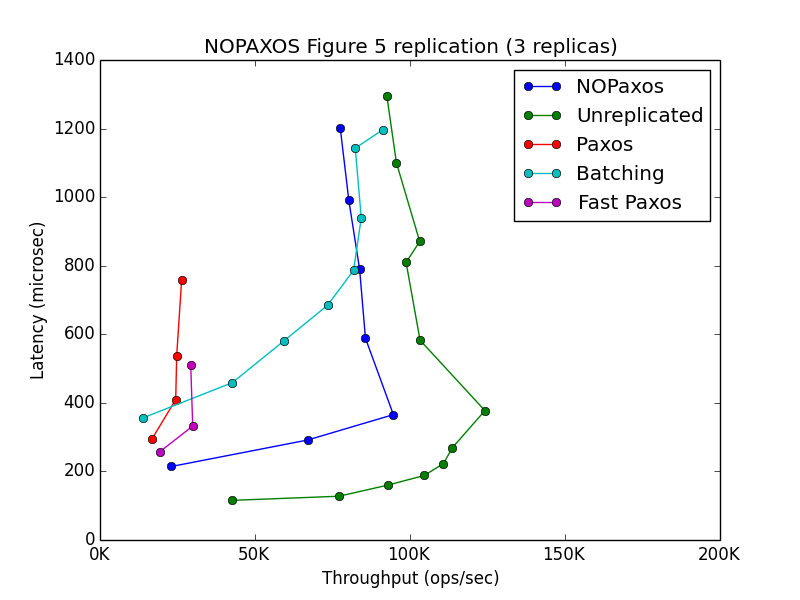
\includegraphics[scale=0.5]{figures/Figure5-3.png}
\caption{Reproduction of Figure 5 in \cite{nopaxos} with 3 replicas, showing latency vs. throughput comparison for NOPaxos and other protocols}
\end{figure}

Our results with 3 replicas (shown in Figure 5) are much closer those of the original paper. In particular, although NOPaxos still does not perform as well as unreplicated, it achieves the highest throughput with the lowest latency of any of the consensus protocols. Thus even though NOPaxos does not perform as well on a cloud platform as on dedicated hardware, it still performs better than other consensus protocols when only 3 replicas are used, and therefore could be a useful mechanism for replication in the cloud in select situations. 

\subsection{Analysis of Bottleneck} \label{bottleneck}

We saw in Figures 3 and 4 that NOPaxos on a cloud platform encounters a bottleneck not present (or at least less evident) on dedicated hardware. Our initial hypothesis was that this bottleneck was a result of the modifications necessary for NOPaxos to run on a cloud platform, specifically the requirement that multicast be implemented in software rather than in the network. This hypothesis was supported by our Figure 4 results, which indicated that adding more replicas impacted performance in a way not seen on dedicated hardware; this could easily be related to the need create an extra copy (in software) of every packet and send it to each replica. 

We therefore set up an experiment to verify that the bottleneck of the system was at the sequencer node (where software multicast was implemented). We already could trivially tell from our earlier results that the bottleneck could not be at the clients, as the clients followed the same procedure regardless of the consensus protocol being tested and achieved a higher throughput with unreplicated. Thus we had only to determine whether the bottleneck lay at the sequencer node or at the replicas. Recall that the sequencer node forwards packets to the replica nodes. We therefore knew that if the system bottleneck was at the replicas rather than the sequencer, then the throughput at the sequencer node would be higher than the throughput of the overall system. 

\begin{figure}[tp]
\centering
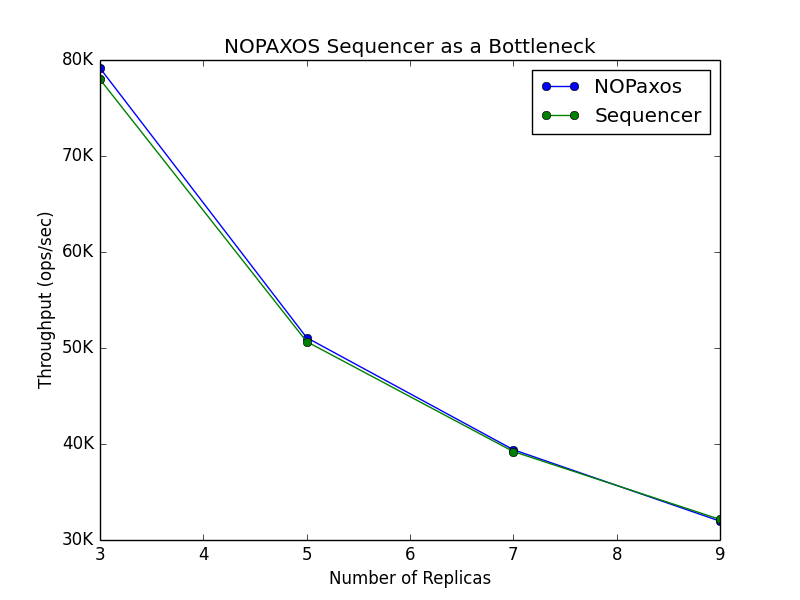
\includegraphics[scale=0.5]{figures/final_SeqBottleneck.png}
\caption{Effects of sequencer on NOPaxos throughput, showing maximum throughput of system and sequencer with increasing number of replicas}
\end{figure}

A graph of the throughput of NOPaxos with an increasing number of replicas, both at the sequencer node and for the overall system, is shown in Figure 6. We can see that the throughput of the sequencer dictates the throughput of NOPaxos as a whole closely follows that of the sequencer. We think that any slight difference is the result of the way we took our measurements. This supports our hypothesis that the throughput of the sequencer does, in fact, dictate the throughput of the entire system. 

The sequencer is written in C++ using raw sockets, and so is not easily optimized. We experimented with increasing the sequencer's compute power to see if this improved performance, but we saw no changes, confirming that I/O is the bottleneck. Although future work may improve upon the sequencer and thus improve NOPaxos performance as a whole on cloud platforms, we currently see few, if any, opportunities for optimization at the sequencer. As discussed in \ref{related}, many other consensus protocols that reduce performance overhead either make assumptions about the network or the nature of client requests (i.e. commutativity), suggesting that achieving comparable performance to unreplicated without any assumptions is a fundamentally difficult problem. Thus improvement to the sequencer at this point would take significant investigation and innovation. 